Denne version udgør synopsis for det videre arbejde med en
referencearkitektur. Formålet er at konkretisere et muligt indhold med
henblik på udpegning af interessenter samt at afgrænse opgaven i forhold
til øvrige aktiviteter. Synopsis vil, på kortest mulige form, giver et
overblik over strukturen og indholdet af den endelige arkitektur.
Synopsen er ikke et gennemarbejdet bud på den endelige løsning, men skal
udtale sig om retning og afprøve rammerne for det videre arbejde.

\section{Introduktion}\label{introduktion}

\subsection{Formål}\label{formuxe5l}

Referencearkitekturen understøtter anvendelse og udviklingen af
offentlige it-systemer, der

\begin{itemize}
\tightlist
\item
  (gen)anvender oplysninger til sagsbehandling eller selvbetjening
\item
  sender eller modtager meddelelser fra andre it-systemer
\end{itemize}

\subsection{Scope}\label{scope}

Referencearkitekturen beskriver anvendelse af og udvikling af it-system
der reguleres af blandt andet:

\begin{description}
\tightlist
\item[EU databeskyttelse]
\emph{lov} som beskriver pligter og rettigheder ved behandling af
persondata
\item[EU eIDAS]
\emph{lov} som definerer registrede tillidstjenester
\item[Persondata lov]
\emph{lov} som beskriver pligter og rettigheder ved behandling af
persondata
\item[Lov om Digital Post]
\emph{lov} der gør det obligatorisk for virksomheder og borgere at
modtage digitale meddelelser fra offentlige afsendereß
\end{description}

Referencearkitekturen skrives på baggrund af den fællesoffentlige
digitaliseringsstrategi 2020 under initiativ 8.1 med tilslutning fra FM,
UFM, EVM, SIM, JM, EFKM, MBUL, SÆM, SKM, MFVM, BM, KL og Danske Regioner

\begin{quote}
For at operationalisere, hvilke krav hvidbogen konkret stiller til
initiativer og systemer udarbejdes en referencearkitektur for deling af
data og dokumenter, der blandt andet beskriver fælles behovsmønstre og
mønstre for teknisk understøttelse, herunder de forskelige roller, der
skal afklares i initiativerne. Referencearkitekturen udpeger også
eventuelle områder for eksisterende og nye fælles standarder og
infrastruktur, som skal lette initiativernes implementering.
Referencearkitekturen bliver således en generel ramme og støtte for alle
initiativernes egen specifikke arkitektur.
\end{quote}

Uden for scope:

\begin{itemize}
\tightlist
\item
  åbne data, der ikke kræver adgangskontrol
\item
  registrering og anvendelse hos registerejer
\end{itemize}

\subsection{Centrale begreber}\label{centrale-begreber}

I det efterfølgende vil begrebet data blive brugt til at betegne både
oplysninger på dokumentform og oplysninger der optræder i registre. Vi
anvender begrebet datasamling både om et register og et repository med
dokumenter.

\begin{figure}
\centering
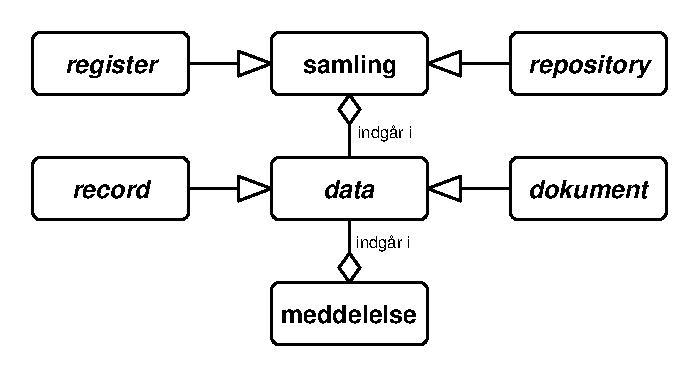
\includegraphics{abstraktion.pdf}
\caption{Anvendelse af begrebet data og relaterede begreber i denne
referencearkitektur}
\end{figure}

\subsection{Anvendelse}\label{anvendelse}

Referencearkitekturen skal

\begin{itemize}
\tightlist
\item
  danne et fælles sprog til at formulere en fælles handlingsplan
\item
  bruges som reference ved løsningsbeskrivelser
\end{itemize}

\subsection{Tilblivelse og governance}\label{tilblivelse-og-governance}

Første udgave er skrevet hos Kontor for Data og Arkitektur af Mads
Hjorth, Digitaliseringsstyrelsen og Anders Fausbøll, Omnium IT.

Endelig godkendelse forventes hos Styregruppe for Data og Arkitektur
under Digitaliseringsstrategien 18. december 2018.

\subsection{Metoderamme}\label{metoderamme}

Skrives indefor rammerne af Fællesoffentlige Digital Arkitektur, det vil
sige; erfaringer fra OIO referencearkitektur, EIRA, TOGAF, ArchiMate.

\subsection{Relation til andre
referencearkitekturer}\label{relation-til-andre-referencearkitekturer}

Gør brug af

\begin{itemize}
\tightlist
\item
  Fællesoffentlig referencearkitektur for brugerstyring
\end{itemize}

Skal kunne anvendes af

\begin{itemize}
\tightlist
\item
  Fællesoffentlig referencearkitektur for selvbetjening
\item
  Fællesoffentlig referencearkitektur for overblik over egne sager
\end{itemize}

Skal anvendes i kontekst sammen med

\begin{itemize}
\tightlist
\item
  Deling af dokumenter på sundhedsområdet
\item
  Indberetning til registre på sundhedsområdet
\item
  Sag- og dokument på det kommunale område
\end{itemize}

\section{Strategi}\label{strategi}

\subsection{Forretningsmæssige
tendenser}\label{forretningsmuxe6ssige-tendenser}

\begin{itemize}
\tightlist
\item
  Ensretning og nationale indsatser
\item
  Data øget værdi for organisationer
\item
  Øget bevågenhed omkring beskyttelse af privatliv
\item
  Øget opmærksomhed om håndtering af personlige oplysninger
\item
  Mængden af oplysninger der håndteres stiger
\item
  Grænseoverskridende services
\end{itemize}

\subsection{Teknologiske tendenser}\label{teknologiske-tendenser}

\begin{itemize}
\tightlist
\item
  øget central standardisering af begreber, datamodeller og grænseflader
\item
  Flere og mere forskelligartede enheder forbundet til netværket
\item
  Øgede forventninger til brugervenlighed af offentlige digitale
  services
\item
  Mængden af tilgængelige oplysninger vokser
\item
  Arkitekturvision for anvendelse og udstilling
\item
  Intergrated Service Delivery
\item
  ''Ineroperability/Samarbejdende infrastrukturer / Økosystem af fælles
  løsninger?''
\item
  ''Valgfri for anvender mellem flere tekniske udbydere af samme
  oplysninger''
\end{itemize}

\subsection{Strategiske målsætning}\label{strategiske-muxe5lsuxe6tning}

{[}beskriv målsætninger i eksisterende aftaler og strategier, også gerne
fra andre områder{]}

\begin{description}
\tightlist
\item[Interoperability]
\emph{mål} om sammenhængende services\ldots{} integrated service
delivery
\item[Once-only]
\emph{mål} om at borger og virksomhed kun skal afgive den samme
information til det offentlige en gang\ldots{} (men give lov til
genbrug?)
\item[Transperancy]
\emph{mål} om borger og virksomheder skal kunne se hvilke data der
findes om dem og hvor disse data anvendes
\item[Re-use]
\emph{mål} om genbrug af it med henblik på lavere omkostninger
\end{description}

\subsection{Vision}\label{vision}

{[}fokus på første workshop{]}

\begin{quote}
\emph{data deles på en måde hvor dataejer ikke unødigt begrænser
genbrug\ldots{}} \emph{(prøve at ramme høste-så problemet og sikre
gennemsigtighed og beskyttelse)} \emph{Nemmere at bruge og sværere at
misbruge}
\end{quote}

\subsection{Værdiskabelse}\label{vuxe6rdiskabelse}

\begin{itemize}
\tightlist
\item
  Mindre besvær for borger og virksomheder ved brug af digitale services
\item
  Simplere arbejdsgange og mere potentiale for automatisering hos
  myndigheder {[}og virksomheder{]}
\item
  Understøtte transparens og bevare tillid til registre
\item
  Effektiv systemudvikling (begrænse udfaldsrum, opsamle best practice)
\end{itemize}

\subsection{Strategiske principper}\label{strategiske-principper}

\begin{itemize}
\tightlist
\item
  F1: Autoritative register med henvisninger til andre registre
\item
  F2: Ansvar for begrænsning af adgang ligger hos registerejer
\item
  I1: Fælles referenceinformationsmodel
\item
  I2: Dokument-princip (attester mv.)?
\item
  A1: Onlineopslag i sagsbehandling og selvbetjening
\item
  A2: Log adgang
\item
  A3: Adgang til og fra internationale registre sker gennem national
  gateway
\item
  T1: Central fuldmagt/rettighedsstyring
\item
  T2: Multi-flavour-api
\end{itemize}

\section{Forretning}\label{forretning}

\subsection{Aktører}\label{aktuxf8rer}

\begin{itemize}
\tightlist
\item
  Offentlig myndigheder, og virksomheder der handler på vegne af dem.
\item
  Borger og virksomheder
\end{itemize}

\subsection{Opgaver}\label{opgaver}

Referencearkitekturen finder anvendelse i løsningen af alle offentlige
opgaver.

\begin{itemize}
\tightlist
\item
  Borger og virksomhedsvendte selvbetjeningsløsninger
\item
  Myndigheders sagsbehandling
\item
  Tværgående analyse, tilsyn, kontrol
\end{itemize}

\subsection{Funktioner}\label{funktioner}

Referencearkitekturen beskriver tre centrale use cases hvor aktører
arbejder sammen i forskellige roller

\begin{figure}
\centering
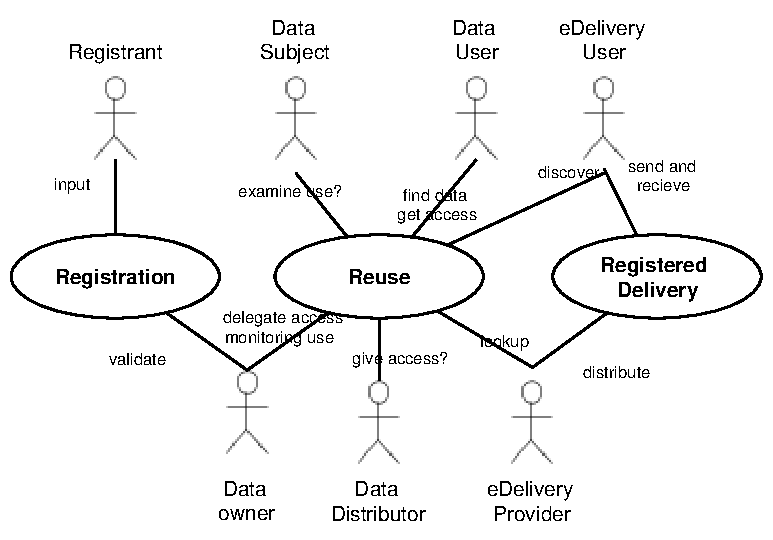
\includegraphics{usecases.pdf}
\caption{Tværgående use cases og funktioner hos de enkelte roller}
\end{figure}

Registrering \textasciitilde{} \emph{collaboration} hvor oplysninger
bringes på digital form

Datanvendelse \textasciitilde{} \emph{collaboration} hvor oplysninger
anvendes i en opgave

Registreret forsendelse \textasciitilde{} \emph{collaboration} hvor
meddelelser sendes uafviseligt

\subsection{Roller}\label{roller}

Nogle er specialisering af Databehandler\ldots{} {[}tilføj kilder til
roller{]}

\begin{description}
\tightlist
\item[Registrant]
\emph{rolle} som bringer oplysninger på digital form, registrer
\item[Datasubject]
\emph{rolle} som oplysninger handler
\item[Dataanvender]
\emph{rolle} der anvender oplysninger fra et register
\item[eDelivery kunde/forbruger?]
\emph{rolle} som der sender og modtager meddelelser
\item[Dataejer]
\emph{rolle} som ejer registreringer/data, ansvar for at udarbejde
adgangspolitik
\item[Datadistributør]
\emph{rolle} som ejer registreringer/data, ansvar for at udarbejde
adgangspolitik
\end{description}

\subsection{Tværgående processer (proces-trin, business
functions?)}\label{tvuxe6rguxe5ende-processer-proces-trin-business-functions}

Herunder beskrives hvor de enkelte business functions hos de enkelte
roller anvendes i kontekst af nogle generiske procesmønstre.

\begin{itemize}
\tightlist
\item
  Sagsbehandling (fra sag og dokument):
\item
  Simpel selvbetjening (fra selvbetjening):
\item
  Tværgående selvbetjening (fra sammenhængende services):
\item
  Indsigt i oplysninger og deres anvendelse (fra overblik?)
\item
  Sende meddelelse (tilmeldingslister)
\item
  Modtage meddelelse (måske påmindelser)
\item
  Tag et dokument med til en anden service provider (der ikke har adgang
  til registre) Beskrive hvordan dokumenter valideres.
\end{itemize}

\subsection{Forretnings-tjenester?
-funktioner?}\label{forretnings-tjenester--funktioner}

Procestrin kan realiseres af interne busines functions eller trække på
eksterne business services. Skal vi bare slå services og functions
sammen (da vi ikke taler om implementering endnu)

{[}Vi skal være bedre til at beskrive hvordan vi trækker på elementer
fra brugerstyring, men husk at holde det teknologi-fri{]}

\subsection{Forretningsobjekter}\label{forretningsobjekter}

{[}Bør identificeres på workshop. Skal det være begrebsmodellering eller
logiske kernemodeller?{]}

\subsubsection{Data}\label{data}

Abstrakt\ldots{}bruges om både registerrecord og dokument

\subsubsection{Registeroplysning
(record)}\label{registeroplysning-record}

\subsubsection{Dokument}\label{dokument}

{[}Dokument model fra OIO{]}

\subsubsection{Datasamling}\label{datasamling}

{[}Datasæt model{]}

\subsubsection{Datasubjekt}\label{datasubjekt}

{[}Grunddata person{]}

\subsubsection{Model/Schema}\label{modelschema}

{[}Modelregler fra FDA{]}

\subsubsection{Meddelelse}\label{meddelelse}

{[}NgDP{]}

\subsubsection{Påmindelse}\label{puxe5mindelse}

{[}NgDP{]}

\subsubsection{Registreringshændelse?}\label{registreringshuxe6ndelse}

{[}Datafordeler{]}

\section{Teknik}\label{teknik}

forretningsfunktionerne understøttes/realiseres af applikationer.

\subsection{Applikationsroller}\label{applikationsroller}

\subsubsection{eDelivery Service
Provider}\label{edelivery-service-provider}

som skal kunne: - udstille eller levere meddelelser til modtager -
modtage og distribuere meddeleleser - fortælle andre om deres kunder

\subsubsection{Dataservice}\label{dataservice}

som skal kunne: - opbevare datasamling - begrænse adgang til de rigtige
- måske vedligeholde og udsende abonnementer

\subsubsection{Kontaktregister}\label{kontaktregister}

som er en slags data service med en særlig type oplysninger

\subsubsection{Log}\label{log}

som er en slags data service med særlige oplysninger

\subsubsection{Indeks}\label{indeks}

som er en slags data service med særlige oplysninger kan undværes, men
ikke effektivt.

\subsection{Katalog}\label{katalog}

som ikke er en dataservice fordi der ikke er begrænset adgang

kan undværes, men ikke effektivt.

{[}Skal vi have en ``beskyttet dataservice'' og en offentlig?{]}

\section{Tekniske Implementering(er)}\label{tekniske-implementeringer}

Her grupperes de enkelte roller og applikationsroller jf forskellige
mønstre.

\subsection{Datanvendelse}\label{datanvendelse}

Når myndighed vil have adgang til data hos en anden er det er par
mønstre

\subsubsection{Direkte adgang, SOA}\label{direkte-adgang-soa}

\subsubsection{Datadistribution}\label{datadistribution}

sammenstilling samt adgangskontrol og logning

\subsubsection{Distribueret Service- og
data-platform}\label{distribueret-service--og-data-platform}

\subsection{Registreret forsendelse}\label{registreret-forsendelse}

Når en myndighed vil sende noget til en myndighed, virksom eller borger.

\subsubsection{SOA / Email\ldots{}}\label{soa-email}

\subsubsection{Fælles system}\label{fuxe6lles-system}

e.g.~e-Boks.

\subsubsection{Service Providers}\label{service-providers}

kan være både generisk eller specifik for et domæne.

\subsection{Registrering}\label{registrering}

skal med for at forklare index

\subsubsection{ansvar hos registrant}\label{ansvar-hos-registrant}

\subsubsection{ansvar hos dataejer}\label{ansvar-hos-dataejer}

\subsubsection{ansvar hos distributør?}\label{ansvar-hos-distributuxf8r}

\subsection{Områder for
standardisering/profileringer}\label{omruxe5der-for-standardiseringprofileringer}

(Per mønster?, matrix) - Service Design Guidelines - Access Protocols -
Distribution Protocols - Synchronisation Protocols

\begin{itemize}
\tightlist
\item
  Metadata for opslag/søgning/anvendelse
\item
  Log format
\item
  Identifikation
\item
  Klassifikation af følsomhed
\item
  Klassifikation af anvendelse (sagsbehandling vs analyse)
\item
  Hændelsesbeskeder
\item
  Protokol for flytning af filer, kryptering
\item
  Hjemmel (samtykke, lov)
\item
  Context
\end{itemize}

\subsection{Identifikation af eksisterende
standarder}\label{identifikation-af-eksisterende-standarder}
